\input ../preamble

\begin{document}

{\Huge

  \centerline{\bf TTIC 31230, Fundamentals of Deep Learning}
  \bigskip
  \centerline{David McAllester, Winter 2018}
  \vfill
  \centerline{\bf Rate-Distortion Autoencoders}
  \vfill



%these slides need more detail.  Every slide should be at least doubled.
% it also needs more material.  A theorem on noise in latent variables would be nice.


\slide{Rate-Distortion Autoencoders}

Given an image or sound wave $y$ we can compress it into a coded form $C_\Phi(y)$.

\vfill
Let $|C_\Phi(y)|$ denote the number of bits in the compressed form $C_\Phi(y)$.

\vfill
We let $\hat{y}_\Phi(C_\Phi(y))$ be the decompression of $C_\Phi(y)$.

\vfill
We let $D(y,\hat{y})$ be a measure of the difference between $y$ and $\hat{y}$ (the loss or ``distortion'').

\slide{Rate-Distortion Autoencoders}

$$\Phi^* = \argmin_\Phi \;E_{y \sim \pop}\;|C_\Phi(y)| + \lambda D(y,\hat{y}_\Phi(C_\Phi(y)))$$

\vfill
It is common to take

$$D(y,\hat{y}) = ||y-\hat{y}||^2 \hspace{4em}(L_2)$$

\vfill
or

$$D(y,\hat{y}) = ||y-\hat{y}||_1 \hspace{4em} (L_1)$$

\slide{Conditional Rate-Distortion Autoencoders}

$$\Phi^* = \argmin_\Phi \;\;E_{(x,y) \sim \pop} \;\;\; |C_\Phi(y|x)|\; + \; \lambda D(y\;|\;\hat{y}_\Phi(x,C_\Phi(y|x)))$$

\slide{Colorization}

\centerline{\includegraphics[height = 2in]{../images/colorization}}

\vfill
$${\color{red} \Phi^* = \argmin_\Phi E_{(x,y) \sim \mathrm{Pop}}\;|C_\Phi(y|x)| + \frac{1}{2}\lambda ||y - \hat{y}_\Phi(x,C_\Phi(y|x))||^2}$$

\vfill
If the image can be segmented based on $x$ then $C_\Phi(y|x)$ can be a specification of color of each segment --- this would be very compact.

\slide{A Case Study in Image Compression}

{\bf End-to-End Optimized Image Compression, Balle, Laparra, Simoncelli, ICLR 2017.}

$${\color{red} \Phi^* = \argmin_\Phi E_{y \sim \mathrm{Pop}}\;|C_\Phi(y)| + \frac{1}{2}\lambda ||y - \hat{y}_\Phi(C_\Phi(y))||^2}$$

\anaslide{JPEG at 4283 bytes or .121 bits per pixel}

\bigskip
\centerline{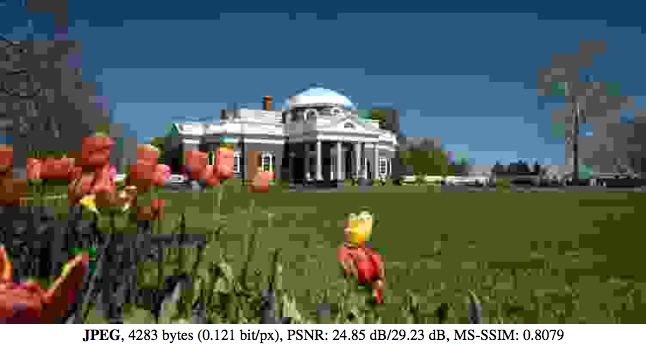
\includegraphics[height=5in]{../images/RateDist2}}

\anaslide{JPEG 2000 at 4004 bytes or .113 bits per pixel}

\bigskip
\centerline{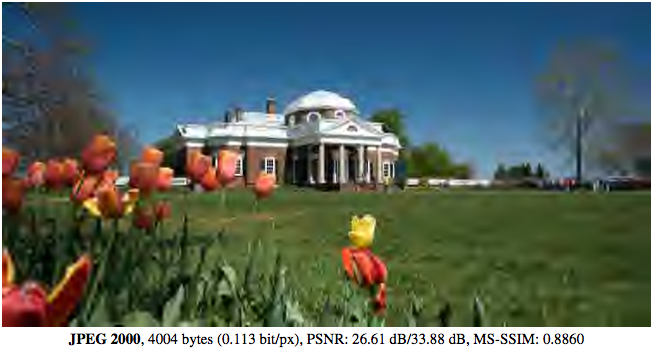
\includegraphics[height= 5in]{../images/RateDist3}}

\anaslide{Proposed Method at 3986 bytes or .113 bits per pixel}

\bigskip
\centerline{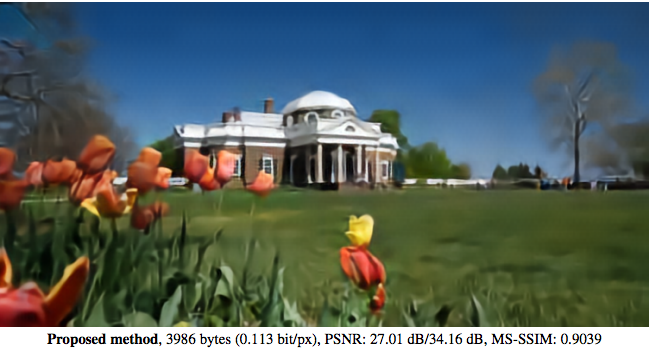
\includegraphics[height = 5in]{../images/RateDist4}}

\slide{The Encoder $C_\Phi(y)$}

This paper uses a three layer CNN for the encoder.

\vfill
The first layer is computed stride 4.

\vfill
The two remaining layers are computed stride 2.

\vfill
They use a generilized divisive normalization (GDN) layer rather than an activation function. 

$$y'[i,j,c] = \frac{y[i,j,c]}{\left(\beta_c + \sum_{c'} \gamma_{c,c'}\; y[i,j,c']^2 \right)^{1/2}}$$

\vfill
$\beta_c$ and $\gamma_{c,c'} = \gamma_{c',c}$ are trained.

\slide{The number of numbers}

\vfill
The first layer is computed stride 4.

\vfill
The next two layers are computed stride 2.

\vfill
Final image dimension is reduced by a factor of 16 with 192 channels per pixel (192 channels is for color images).

\vfill
$$192 < 16 \times 16 \times 3 = 768$$

\vfill
These 192 numbers are rounded to integers.

\vfill
The 192 integers are coded losslessly using $P^{\mathrm{code}}_\Theta$.

\slide{Increasing Spatial Dimension in Decoding}

\centerline{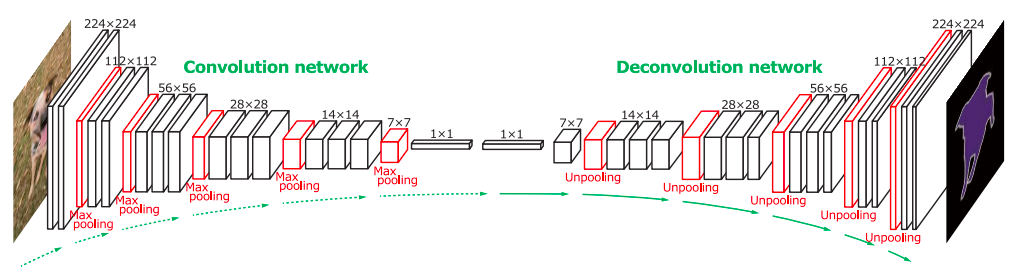
\includegraphics[width=9in]{../images/Deconv}}
\centerline{[Hyeonwoo Noh et al.]}

\slide{Increasing Spatial Dimensions in Deconvolution}

Consider a stride 2 convolution
\begin{eqnarray*}
  y[i,j,c_y] & = &   W[\Delta i, \Delta j, c_x, c_y] x[2i + \Delta i, 2j + \Delta j, c_x] \\
  y[i,j,c_y] & \pluseq & B[c_y]
\end{eqnarray*}

\vfill
For deconvolution we use stride 1 with 4 times the channels.
\begin{eqnarray*}
  \hat{x}[i,j,c_{\hat{x}}] & = &   W'[\Delta i, \Delta j, c_{\hat{y}}, c_{\hat{x}}] \hat{y}[i + \Delta i, j + \Delta j, c_{\hat{x}}] \\
  \hat{x}[i,j,c_{\hat{x}}] & \pluseq & B[c_{\hat{x}}]
\end{eqnarray*}

\vfill
The channels at each lower resolution pixel $\hat{x}[i,j]$ are divided among four higher resolution pixels.

\vfill
This is done by a simple reshaping of $\hat{x}$.


\slide{The Decoder}

This is a deconvolution network of the same architecture with independent parameters.

\vfill
There is a special parameterization of the ``inverter'' for the normalization layer.

\slide{Rounding the Numbers}

We let $C_\Phi(x)$ be the unrounded numerical representation and $\tilde{C}_\Phi(x)$ be the result of rounding.

\vfill
$$\tilde{C}_\Phi(x)_i =  \mathrm{round}(C_\Phi(x)_i) = \lfloor C_\Phi(x)_i + 1/2\rfloor$$

\vfill
Each integer channel of the final layer is coded independently.

\vfill
Context-based adaptive binary arithmetic coding framework (CABAC; Marpe, Schwarz, and Wiegand, 2003).

\slide{Training}

We now have the optimization problem

$$\Phi^* = \argmin_\Phi\; E_{y \sim \mathrm{Pop}} - \log_2 P_\Phi({\color{red} \tilde{C}_\Phi(y)}) + \lambda ||y - \hat{y}_\Phi({\color{red} \tilde{C}_\Phi(y)})||^2$$

\vfill
Issue: The rounding causes the gradients for $\Phi$ to be zero.

\slide{Modeling Rounding with Noise}

$$\Phi^* = \argmin_\Phi\; E_{y \sim \mathrm{Pop}} - \log_2 P_\Phi({\color{red} \tilde{C}_\Phi(y)}) + \lambda ||y - \hat{y}_\Phi({\color{red} \tilde{C}_\Phi(y)})||^2$$

\vfill
At train time (but not test time) the rounding is replaced with additive noise.

\vfill
$$\Phi^* = \argmin_\Phi\; E_{y,\epsilon} - \log_2 P_\Phi({\color{red} C_\Phi(y) + \epsilon}) + \lambda ||y - \hat{y}_\Phi({\color{red} C_\Phi(y)+ \epsilon})||^2$$

\vfill
$$\epsilon_i \;\mbox{drawn uniformly from $[-1/2,\;1/2]$}$$

\vfill
$P_\Phi$ defines a piecewise linear density for each coordinate of $z$. 

\slide{Noise vs. Rounding}

\centerline{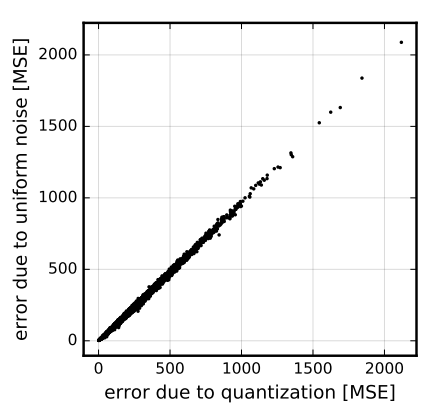
\includegraphics[height=5in]{../images/RateDist5}}

\slide{Differential Entropy vs. Discrete Entropy}

\bigskip
\centerline{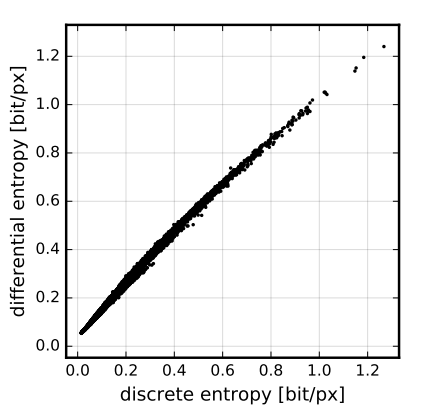
\includegraphics[height=5in]{../images/RateDist6}}

\slide{Varying the Level Of Compression}

$$\Phi^* = \argmin_\Phi\; E_{y \sim \mathrm{Pop}} - \log_2 P_\Phi(\tilde{C}_\Phi(y)) + \frac{1}{2}{\color{red} \lambda} ||y - \hat{y}_\Phi(\tilde{C}_\Phi(y))||^2$$

\vfill
Different levels of compression correspond to different values of $\lambda$.

\vfill
In all levels of compression we replace 768 numbers by 192 numbers.

\vfill
Higher levels of compression result in more compact distributions on the 192 numbers.
\slide{END}

}
\end{document}

